%!TEX root=../tax-democracy-held.tex
%quote needed

%here, now, comes the first-order normative criteria:
%what would make it nice?

% What makes a more efficient, more equitable tax?
% This concerns the conceptual and normative building blocks of taxation.
%Sufficient analytical clarification on a “new understanding of tax”, with particular regard to the PCT has been reached (McCaffery 2002).

%add on "property" Simons' argument that it's 90 percent background conditions, and Offes (2009 via Bosch) addition that rents of cooperation (cf game theory) can, by definition, not be accrued to any one PARTICULAR participant.

To design and choose a normatively superior tax, we need criteria against which to measure alternative regimes.
A normatively superior tax will satisfy and balance \hyperref[sec:tax-optimality]{efficiency} (page \pageref{sec:tax-optimality}) and \hyperref[sec:tax-justice]{equity} (page \pageref{sec:tax-justice}) norms.
It will also be \hyperref[sec:tax-sustainability]{sustainable} (page \pageref{sec:tax-sustainability}) over time.
%this needs to be re-written, the below sections have changed

\section[Optimality]{Optimality:~Desirable Taxes Are Neutral \textsuperscript{\ref{fn:also-in-mpp}}}
	\label{sec:tax-optimality}
%this used to be called efficiency, but I changed the heading.
A system is efficient if it maximizes outputs for given inputs.

%somewhere in McCaffery:
%Ramsey optimal tax literatre:
%"inverse elasticity" rule.
%This can lead to perverse ideas:
%working wifes is ok, but low wages for immigrants with hig hwork ethic?

\paragraph{Which Efficiency Norm?}
But exactly \emph{what} should be maximized?
Efficiency norms vary and can conflict.
I present here three popular definitions in increasing order of strength.
\footnote{
	The selected efficiency principles are all cardinal, rather than ordinal in definition, and do all not consider the aggregation problem commonly known as \emph{diminishing utility to wealth} \citep{Hicks1946}.
	While these are substantial shortcomings, they do not concern me in the efficiency discussion of the perfect tax.
	Respective \emph{equity} implications are discussed in sections \ref{sec:diminishing-marginal-utility} (\hyperref[sec:diminishing-marginal-utility]{diminishing returns}) and \ref{sec:positional-race} (\hyperref[sec:positional-race]{conspicuous consumption}).
}
Earlier entries are subsets of later entries, as visualized in \autoref{fig:Efficiencies}.

\begin{description}
	\item[Pareto Efficiency.]
	\phantomsection
	\label{sec:pareto}
	An allocation is pareto-optimal, when no one can be made better off \emph{without making someone else worse off}.
	Pareto optimality, is, in fact not a pure efficiency norm but includes an equity component, too.

	\item[Kaldor-Hicks Efficiency.]
	\phantomsection
	\label{sec:kaldor-hicks} An allocation is Kaldor-Hicks efficient, when no one can be made better off without making someone else worse off \emph{by the same or a greater amount} of disutility \citep{Kaldor1939,Hicks1939}.
	It can also be described as a pareto-optimal outcome where sufficient compensatory sidepayments can be made from the winners to the loosers.

	\item[Social Welfare Optimum.]
	\phantomsection
	\label{sec:swo} The pure efficiency norm is given by the utilitarian slogan ``The greatest good for the greatest many'' \citep{Mill1863}.
	It knows no equity at all, but is concerned only with the sum total.
	It is also known as a social welfare optimum in game theory (for example, \citealt{Oye-1985-aa}).
\end{description}

\begin{figure}[htbp]
	\centering
	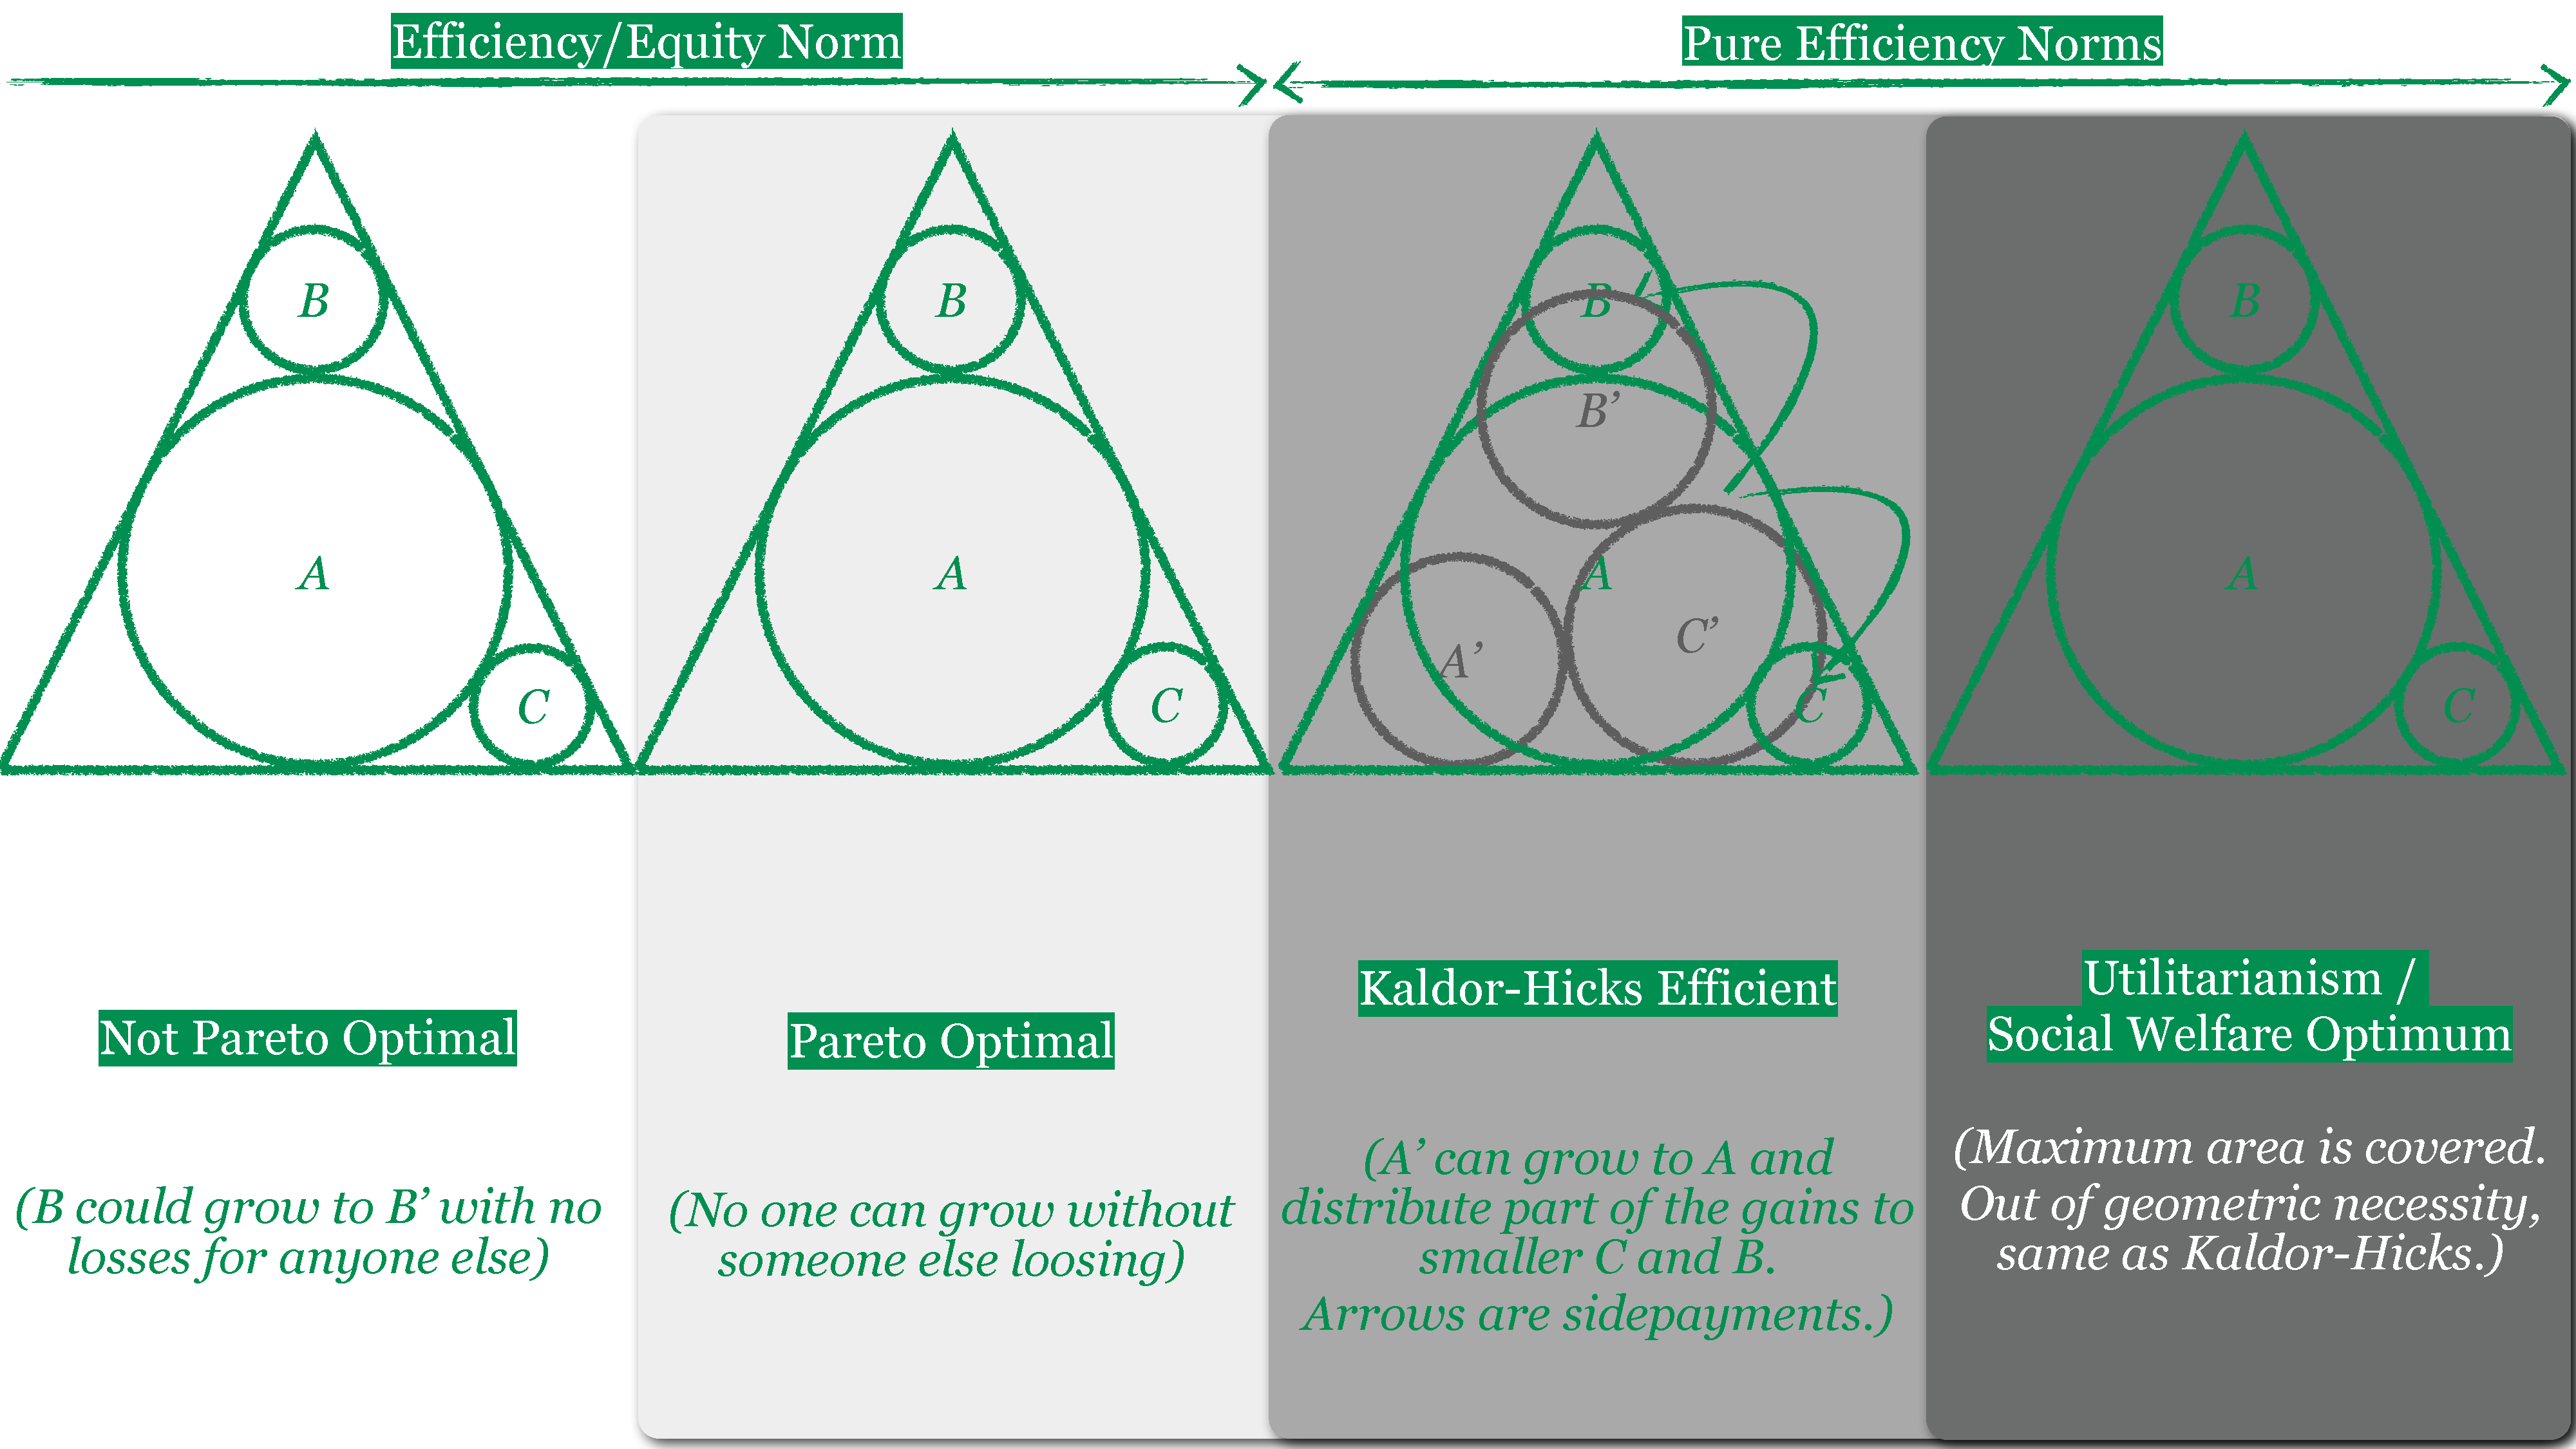
\includegraphics[width=1\textwidth]{efficiency-norms}
	\caption[Selected Efficiency Norms]{Selected Efficiency Norms, Where Area Equals Utility}
	\label{fig:Efficiencies}
\end{figure}

I choose \hyperref[sec:pareto]{Pareto optimality} as the weakest of these efficiency norms and note whenever a stronger efficiency norm is required for an argument.
Pareto efficiency is also widespread efficiency norm that is convenient for its link to \hyperref[sec:perfect-competition]{perfect competition} (page \pageref{sec:perfect-competition}).

\paragraph{In Dubio Pro Mercatus.}
The above posited perfect markets can be shown to work Adam \citeauthor{Smith-1776-lq}'s \emph{Invisible Hand} \citeyearpar{Smith-1776-lq}.
More formally, the first theorem of welfare economics states that any competitive equilibrium will be Pareto optimal:
no one could be made better off, without making someone else worse off\footnote{Demonstrated first graphically by \cite{Lerner1944}, mathematically by \cite{Lange1934}, \cite{Debreu1954} and others.}.

For (\hyperref[sec:pareto]{Pareto}) efficiency, the burden of proof then lies on state interventions in \hyperref[sec:perfect-competition]{competitive markets}. \ref{sec:perfect-competition}
It follows that a tax should affect market interactions as little as possible.

\paragraph{Minimize Deadweight Losses}
The efficiency loss that \emph{does} occur when taxes alter market interactions is called a deadweight loss (DWL), illustrated in \autoref{fig:DWL}.
It arises as follows:
consumers and producers both reduce their buying and selling, as consumers face higher and producers lower prices.
This reduces the welfare, or surplus of consumers and producers.
Some of this loss is transferred to government.
The net that is not recouped as tax revenue is the deadweight-loss of taxation.
%note, improve language-wise:
%DWL is the opposite of gains from trade.

%the question is:
%why is the DWL here, and not in some other section, namely do ability?
%this figure happens earlier as fig:DWL

\begin{desideratum}[Minimal Deadweight Loss]
	A desirable tax should have a minimal deadweight loss.
	\label{des:minimal-DWL}
\end{desideratum}

\begin{desideratum}[Incentives]
	%is this not the same as DWL?
	A desirable tax will maintain and strengthen incentives to maximize private, unobserved effort in work and investment.
	\label{des:Incentives}
\end{desideratum}

%note somewhere that this applies only to revenue generation and redistributive taxation;
%pigouvian is the opposite

\subparagraph{Reformulations of DWL.}
The idea of the DWL of taxation can be reformulated in a number of ways.
\begin{description}
	\item[Factor Unemployment]
	refers to DWLs in markets of factors of production, when tax wedges cause incomplete employment of labor or capital.
	This problem is particularly dire in the indivisible supply of low-productivity labor, where entire strata of workers may be unable to find gainful employment at post-tax wages.
	This problem of \hyperref[sec:StructuralUnemployment]{\emph{structural} unemployment} is further discussed in \autoref{sec:InequalityIsInefficient} and addressed in desideratum \ref{des:low-price-floor}.

	\item[Taxes are Anti-Growth.]
	A sophisticated version of this sentiment will also argue that widespread DWLs waste economic resources in the medium and long run.

	\item[Neutrality.]
	The DWL of a tax can also be described as its impact on a hypothetical, before-tax, pareto optimal market.
	An efficient, desirable tax is neutral in the sense of leaving pre-tax relative prices unchanged \citep[849]{McCaffery2005}.
\end{description}

%\paragraph{Savings Must be Earned.} The discussion of savings here, as elsewhere, concentrates on the trade-off between \emph{saving} and \emph{consuming}.
%However, before money can be either saved or consumed, it has to be earned.
%Another trade-off between \emph{leisure} and \emph{work} applies here.
%Just like saving (desideratum \ref{des:Savings}), this trade-off also has to be adequately incentivized \citep{Frankel1998}.
%In addition to desideratum \ref{des:Savings}:

%introduce work-leisure as a sub-class of DWL or rather, neutrality.
%\begin{desideratum}[Arbitrary Work-Leisure Incentive]
	%A desirable tax should allow for arbitrary, negative incentives for the consumption of leisure.
%	\label{des:leisure}
%\end{desideratum}

%same thing applies to spending and saving
	%is also a sub-class of the DWL
	%consider discussing the OSN and Y2C here, they are sort of exceptions to this rule
	%note that this also has fairness implications that cut both ways.

%maybe the whole issue of capital/agnosticity also belongs in here, maybe this is really just a sub-class of DWL.

%here used to be a section on welfare gains from taxation, but that is now over at mixed economy.

%in here was the section on different kinds of fiscal interventions.
%It has now moved to "mixed economy".

\section[Justice]{Justice:~Desirable Taxes Are Fair}
	\label{sec:tax-justice}
	%this used to be called equity, but that is now in mixed economy
I assume here, axiomatically, that some degree of post-market  equity is desirable.
%further introduction is neeeded

%here, I still have to write a bit on distributive justice
	%http://en.wikipedia.org/wiki/Justice#Theories-of-distributive-justice
	%http://en.wikipedia.org/wiki/Distributive-justice
	%compare them, explain why I go for Rawls

%In philosophy, the term "maximin" is often used in the context of John Rawls's A Theory of Justice, where he refers to it (Rawls (1971, p.
%152)) in the context of The Difference Principle.
%Rawls defined this principle as the rule which states that social and economic inequalities should be arranged so that "they are to be of the greatest benefit to the least-advantaged members of society".
%In other words, an unequal distribution can be just when it maximizes the mininum benefit to those who have the lowest allocation of welfare-conferring resources (which he refers to as "primary goods").[5][6]
	%note that this is only loosely related to the maximin use otherwise used.

%\subsection{Natural Persons}

%The first complication of taxation is actually a clarification:
%redistribution is only meaningfully defined between \emph{natural} persons, that is, actual human beings.
%William \citeauthor{Vickrey1947} begins his classic \emph{Agenda for Progressive Taxation}:
%``Genuinely progressive taxation is necessarily personal taxation'' (\citeyear{Vickrey1947}:
%1).

%comment here somehow on the foundational argument:
%that you are entitled to whatever you earn in uncoerced exchange --- or are you?

%also comment here somehow on where that relies on the state
	%in protection of property rights for private consumption
	%in protection of land etc.
%for control
	%na this isn't so good.

%we know from earlier desiderata, we want it to be progressive, but just how and why we want that is less clear.
%that's why this is about fairness, not just equity.

\subsection[Foundational Arguments]{Foundational Arguments}
%somehow set them up here?
%that stuff that has been earned through uncooerced exchange \ldots
%set myself up for the later foundational arguments on the PCT and the LVT.

\subsection[Distributional Justice (as Fairness)]{Distributional Justice as Fairness:~When is Inequality Unjust?}
%here, I moved two paragraphs of rawls to wanted.
%Transition missing.
\paragraph{Distributional Justice.}
Second, Rawls suggests two distributive norms, the \emph{difference principle} and the \emph{fair equality of opportunity}.
\footnote{
	These two distributive norms follow the equal liberty principle in \emph{lexical} order, meaning that no distributive improvements can justify infringements of equal liberties.
}
Under the \emph{difference principle}, differences in endowments as well as subsequent social and economic inequalities are acceptable only if their granting also benefits the least fortunate.
\footnote{
	\cite[122]{Rawls-1971} warns that this calculus must not only include strictly economic payoffs, but must also take into account the intangible correlates of social inequality as societal and cultural participation, as well as confidence.
}
If inequities cannot be thereby justified, such undeserved differences (by birth or other random allocations) in endowment should be corrected by intervention for \emph{fair equality of opportunity}.

This latter norm of fair equality of opportunity is a pure equity norm on the equality of inputs.

The difference principle is more complicated.
It combines equity and efficiency norms.
It is that weak pareto optimum (WPO),
\footnote{
	An allocation is weakly pareto optimal when no other allocation is \emph{strictly} preferred by everyone.
A strong pareto optimum, by contrast, requires only that all individuals will receive same \emph{or} higher payoffs.
}
which maximizes the minimum payoff (maximin) in outcomes.
\autoref{fig:distributive-norms} illustrates the two Rawlsian norms of distributive justice in context.
%easy to understand formulation required

\begin{figure}[htbp]
	\centering
	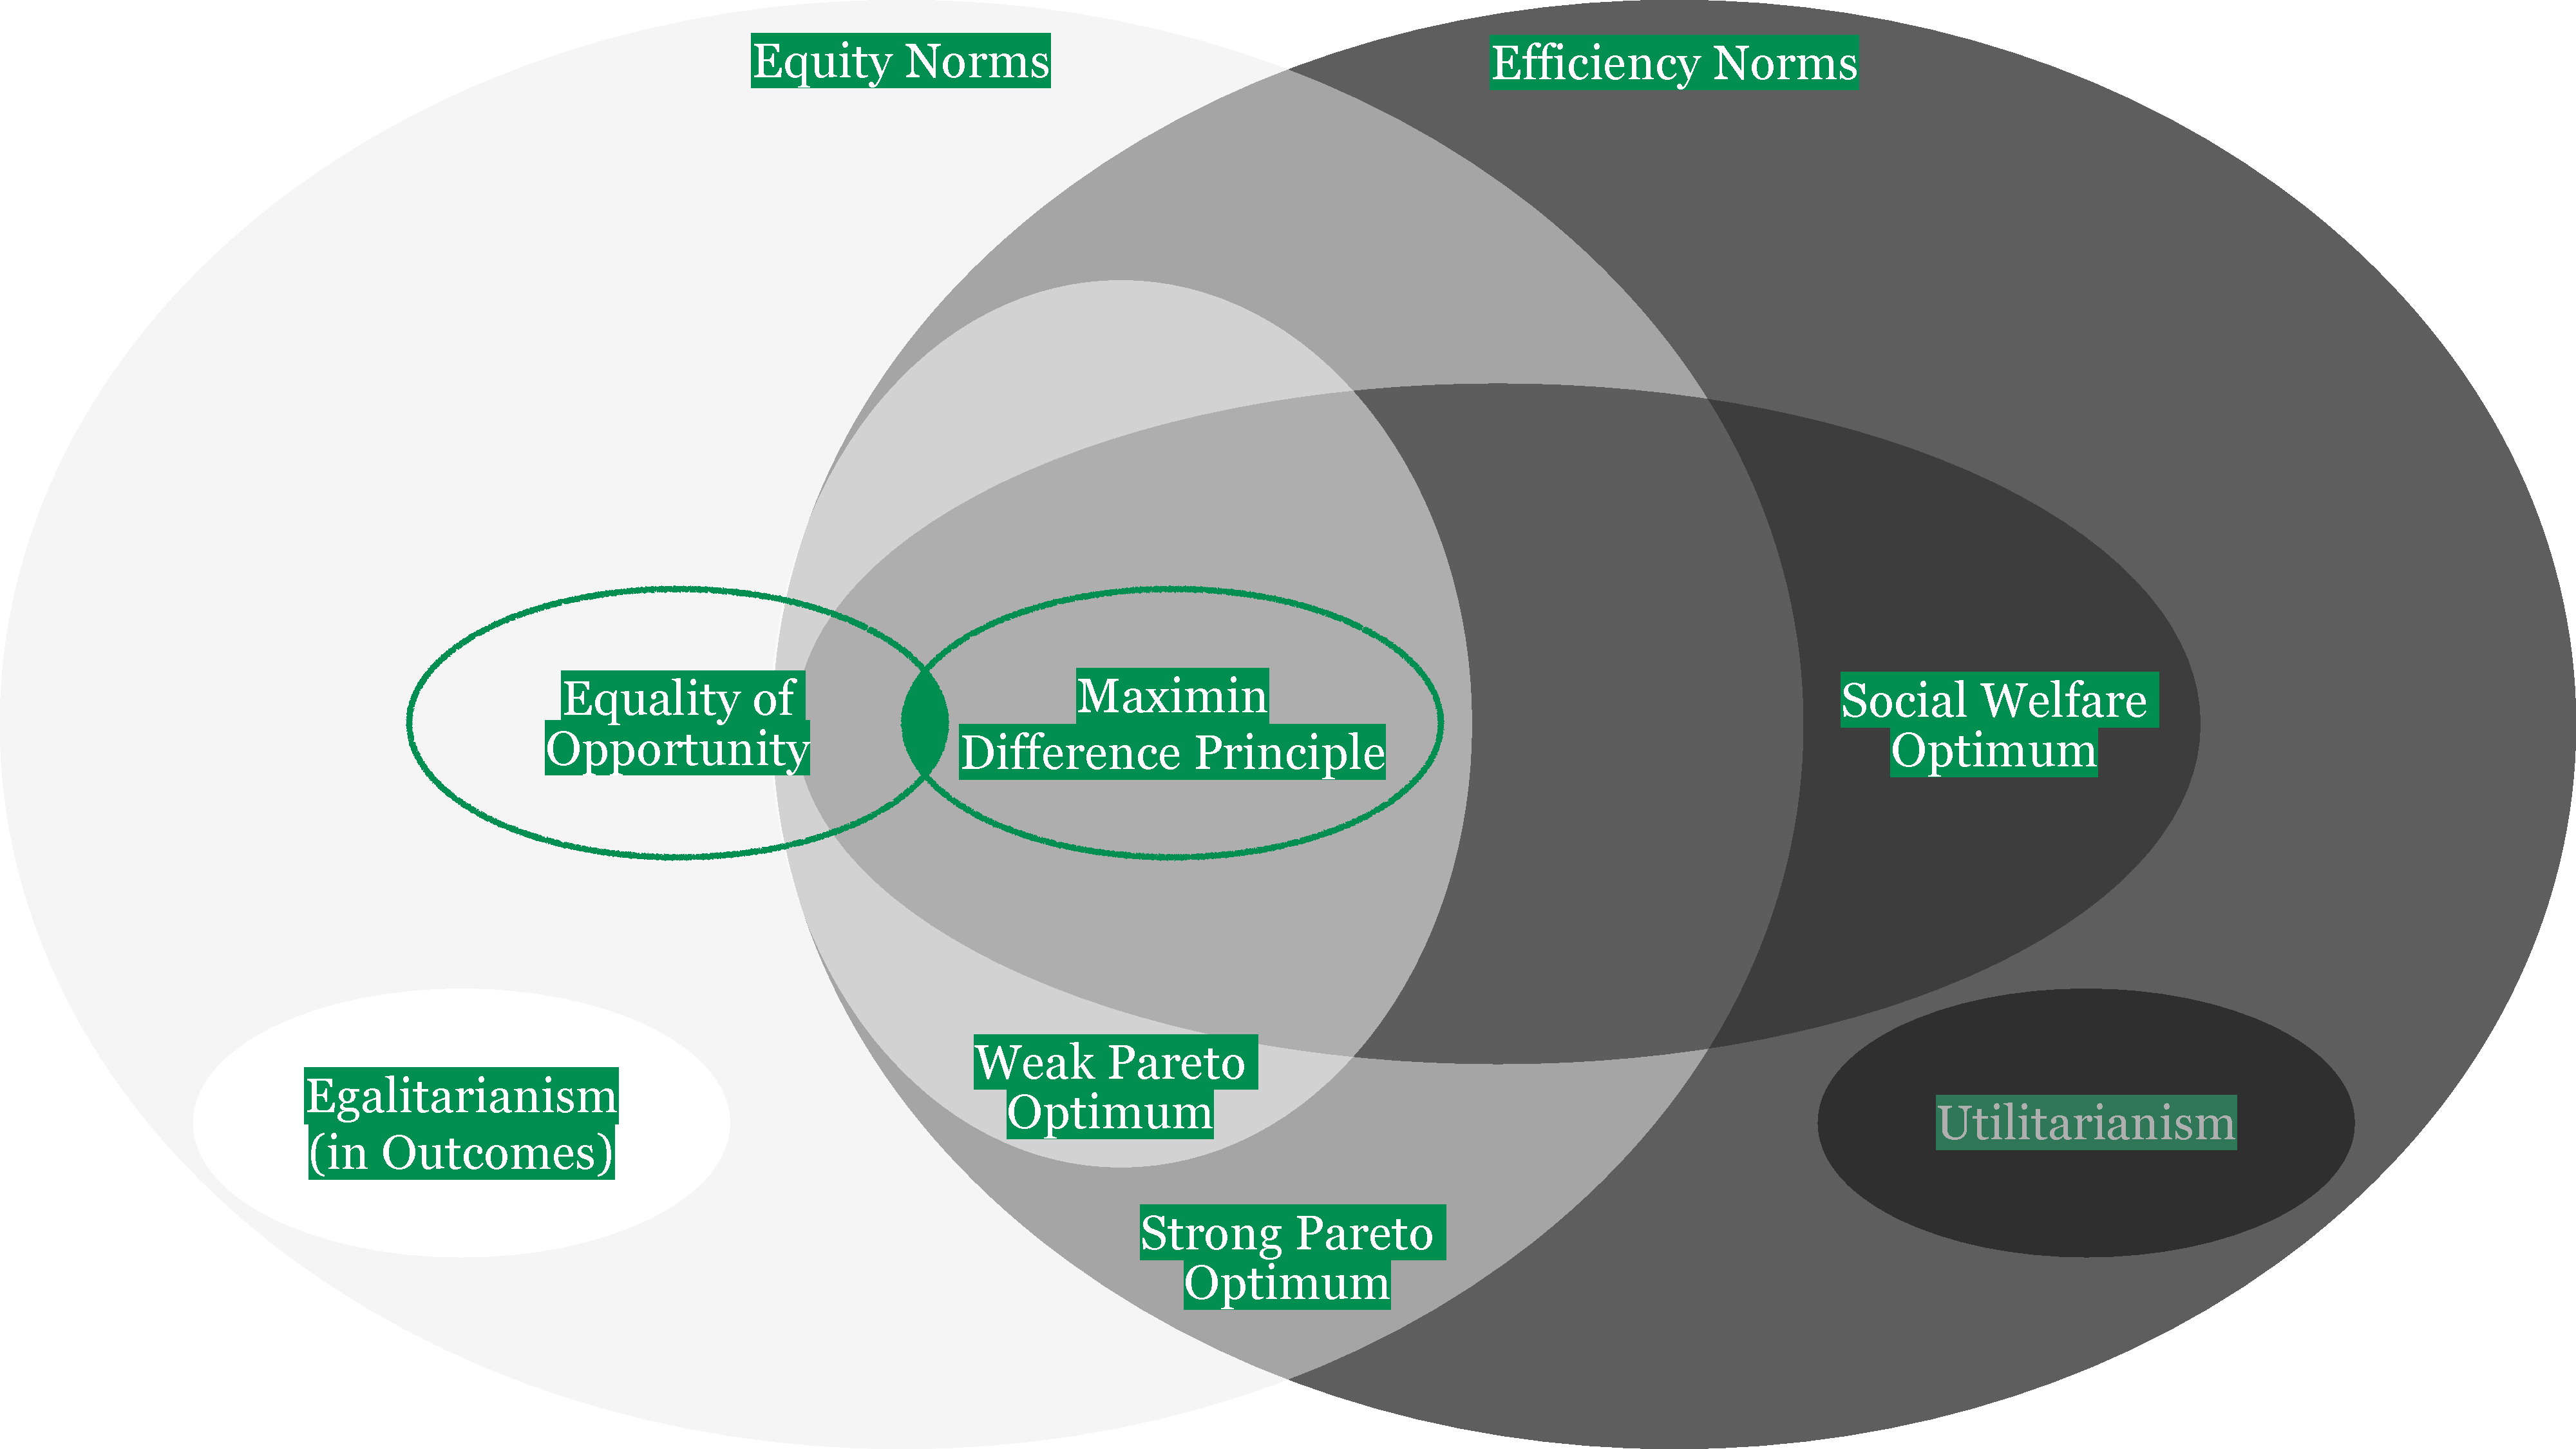
\includegraphics[width=1\textwidth]{distributive-norms}
	\caption[Selected Distributive Norms]{Selected Distributive Norms and Rawlsian Distributive Justice (in green)}
	\label{fig:distributive-norms}
\end{figure}

\paragraph{Why Rawls?}
Any comprehensive discussion of distributional justice is beyond the scope of this thesis.
\citeauthor{Rawls-1971} \emph{Theory of Justice} is presented here for four reasons.

First, \emph{justice as fairness} serves as a convenient cut-off point on a (crudely) imagined continuum of theories of distributive justice from left to right, from egalitarianism to utilitarianism and liberitarianism.
\footnote{
	A right-hand pole comprising of utilitarian \emph{and} libertarian ideals obviously reveals the futility of any one-dimensional scaling of theories of allocative justice.
}
It is assumed that all allocative norms ``left of'' Rawls \citep[such as][]{Cohen2000}, stressing equity over efficiency will strictly prefer the PCT over the status quo.
Conversely, theorists on the right end of the imagined continuum (for instance, \citealt{Nozick1974}) may not share all of the normative foundations of the PCT, or even prefer it over the status quo.

Second, the \emph{difference principle} is \hyperref[sec:foundational-beauty]{invoked} (page \pageref{sec:foundational-beauty}) when I argue the normative superiority of the progressive taxation of consumption.

Thirdly, in arguing that the PCT is the perfect tax, I attempt to establish it as an \emph{reflective equilibrium} \citep[49]{Rawls-1971} emerging from a pragmatic-spirited back-and-forth between what is \hyperref[sec:axiology]{desirable}, and what is \hyperref[sec:ontology]{doable} \citealt[856]{McCaffery2005}.

Fourth, \citeauthor{Rawls-1971}' \emph{Theory of Justice} (\citeyear{Rawls-1971}) is an end-state theory of distributive justice \citep[1007]{Fried1999}, not a procedural prescription (for example \citealt{Dahl-1989-aa}).
%This thesis, likewise, hypothesizes a normatively superior allocative outcome (``Is this the best of all \ldots'', compare page \pageref{sec:Wanted}).
A political process, aside from \citeauthor{Rawls-1971}ian liberty, is not prescribed in its own right.
It merely serves as an \emph{independent} variable in \autoref{chap:no-better-tax},explaining and criticizing why it may have failed to deliver the superior allocative outcome.
	%elaborate this further, Kohler's comment ``your're an economist'', ideas as explanandum may apply here

\paragraph{Implications for Tax Design.}
Two desiderata for tax design emerge from \citeauthor{Rawls-1971}'s Theory of Justice.

First, the principle of \emph{fair equality of opportunity} introduces equity as a goal for taxation.
It is a general and unspecific norm.
Translating it into a desideratum for tax design hinges on an empirical assessment of  opportunity
	%
 in the real world.
A specification of this norm must therefore await an inspection of the \hyperref[sec:inequality-dynamics]{governing dynamics of inequality} (page \pageref{sec:inequality-dynamics}) in modern society. \ref{sec:inequality-dynamics}
%It is provided in desideratum.
	%\ref{des:SharpProgression}
	%does not exist, does not work

Second, the \emph{difference principle} provides a more straightforward guideline for redistributive taxation.
It implies that taxation should exempt from redistribution economic inequality if, and to the extent that, it makes the least fortunate better off.
This may occur when able people require economic \hyperref[des:Incentives]{incentives} to exert maximum efforts (desideratum \ref{des:Incentives}).
%does not work, exist
	%, or when \hyperref[des:Entrepreneurship]{smart investors}, acting in their own self-interest, can be trusted to make good production decisions (desideratum \ref{des:Entrepreneurship}).
Because axiomatically assumed perfectly competitive markets can be shown to be pareto optimal, it follows that:

\begin{desideratum}[Difference Principle]
	\label{des:difference-principle}
	A desirable tax exempts from redistribution economic inequality if, and to the extent that, it makes the least fortunate better off.
\end{desideratum}

Generally, for axiomatically assumed \emph{homo economicus} to \hyperref[sec:perfect-competition]{perfectly compete}, she needs incentives.
Desideratum \ref{des:Incentives} is closely related to desideratum \ref{des:minimal-DWL} (\hyperref[des:minimal-DWL]{minimal DWLs}).

%discuss somewhere:
%vertical vs.\ horizontal equity (\citealt{Mankiw-2004-aa}:
%255);
%this is key for a rule-of-law, fair tax.
%It's also the same norm as gleiches wird gleich, unterschiedlich unterschiedlich behandelt, somewhere in the German Basic Law.
%Find out where.

\section[Sustainability]{Sustainability:~A Desirable Tax Ensures Future Prosperity}
	\label{sec:tax-sustainability}
	%definietely need better title

%think about making this into a catch-all thing:
%capture here both the time-inconsistency stuff as well as the commons failures et al.

%somehow, the savings rate desideratum is missing here.

%also need a standard here, maybe the solow growth stuff?
%not sure.
%or maybe, the standard is simply to have an arbitrary savings rate set by the democratic sovereign?
%no \ldots it must be at least Solow, clearly.

Social and economic systems are dynamic systems:
they evolve over time.
Their change is predominantly \emph{anthropogenic} or \emph{endogenous}, with the exception of very sparse or very slow variations in natural systems.
Tomorrow's economic output will, to the largest extent, be a function of today's economic
	%really?
configuration --- except, of course, if another extinction event hits or another ice age sets in \citep{Courtillot2002}.
\footnote{
	Then again, the jury is still out on whether another anthropogenic ice age is in the making \citep{UnitedNations2007, Rahmsdorf-2009}.
}


It follows that a desirable fiscal allocation should also contribute to sustainability.
I exclude here narrower defined environmental and social dimensions of sustainability and relegate these \hyperref[sec:common-good]{Common Goods} to be internalized through Pigouvian taxation. \ref{sec:common-good}
Instead, I concentrate on pure fiscal sustainability over time, or \emph{intertemporal optimization} in the \hyperref[sec:short-term-inconsistency]{short-} and \hyperref[sec:long-term-inconsistency]{long-}term. \ref{sec:short-term-inconsistency} \ref{sec:long-term-inconsistency}

Sustainability bears both on equity and efficiency.
An equitable policy ensures same (discounted) utility for people living today vs.\ people living in the future.
An efficient policy ensures maximum (discounted) growth over all periods.
As both criteria often overlap in concrete policy issues, they are discussed together here.

How can taxation help us prosper tomorrow and in a generation?
The answer depends on the chosen time horizon.

%\paragraph{Both Equity and Efficiency Apply.} Policy recommendations for intergenerational allocation bear equally on equity \emph{and} efficiency.
%Sustainability is a goal of
%\hyperref[sec:IntertemporalEquity]{\emph{intertemporal equity}}:
%under a pure equity norm, future generations should enjoy the same prosperity as the current generation (this implies zero growth).
%Conversely, growth is a goal of \hyperref[sec:IntertemporalEfficiency]{\emph{intertemporal efficiency}}:
%under a pure, \hyperref[sec:swo]{utilitarian} efficiency norm (page \pageref{sec:swo}), the world economy should expand as fast as exogenously possible (irrespective of generational incidence).

%%%%%%%%%%here comes more stuff from a random document:
%https://docs.google.com/document/d/1uFpQLhFxSPVstd3WjEr_HkFXj_uyANlmvKtBxC3LGC0/edit